%%%%%%%%%%%%%%%%%%%%%%%%%%%%%%%%%%%%%%%%%%%%%%%%%%%%%%%%%%%%%%%%%%%%%%%%%%%%%%%
%
% Tommy P. Keane
% Master of Science Thesis
% Department of Electrical and Microelectronic Engineering
%
% March 2011
%
%
%
% .tex and .sty modified from:
% http://www.ce.rit.edu/studentresources/gradresource/LaTexThesis.zip
%
%%%%%%%%%%%%%%%%%%%%%%%%%%%%%%%%%%%%%%%%%%%%%%%%%%%%%%%%%%%%%%%%%%%%%%%%%%%%%%%

%%%%%%%%%%%%%%%%%%%%%%%%%%%%%%%%%%%%%%%%%%%%%%%%%%%%%%%%%%%%%%%%%%%%%%%%%%%%%%%
%
% CHAPTER 2
%
% SECTION 2
%
%%%%%%%%%%%%%%%%%%%%%%%%%%%%%%%%%%%%%%%%%%%%%%%%%%%%%%%%%%%%%%%%%%%%%%%%%%%%%%%


%%%%%%%%%%%%%%%%%%%%%%%%%%%%%%%%%%%%%%%%%%%%%%%%%%%%%%%%%%%%%%%%%%%%%%%%%%%%%%%
% BEGIN DOCUMENT

First it is necessary to understand digital image systems from a statistical viewpoint, from the capture stage through to the processing stage. Initial digital capture is through the transformation of incident photon energy that is thresholded into digital signals describing what can be referred to as intensity. To capture color information in a typical CCD array (single channel) the Bayer mask is the most prevalent methodology. It is based on the trichromatic theory of color from the scientific understanding of the human visual system \ref{Palmer1999}, by applying the known sensitivity of the human visual system to middle range wavelengths of visible light (green light). Therefore in the Bayer mask there are twice as many green (G) samples as red (R) and blue (B). What is important to note is that in generating the final color image, there is an application of an intensity interpolation method, known as demosaicking. Each pixel, representing a point in image space (the view), that corresponds to a point in the world space (the scene), is only sampling one color (wavelength) of light: R, G, or B. So for a color image the color values in all the other pixels are interpolations of neighboring pixels. See Figures \ref{Bayer1} and \ref{Bayer2} for a visual description of this process.
 
\begin{figure}[!h]
\label{Bayer1}
\centering
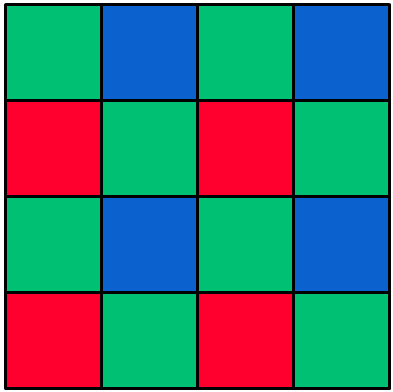
\includegraphics[width=0.3\textwidth]{Bayer1}
\caption{The Bayer pattern image resultant from the bayer filter capture.}
\end{figure}
 
\begin{figure}[!h]
\label{Bayer2}
\centering
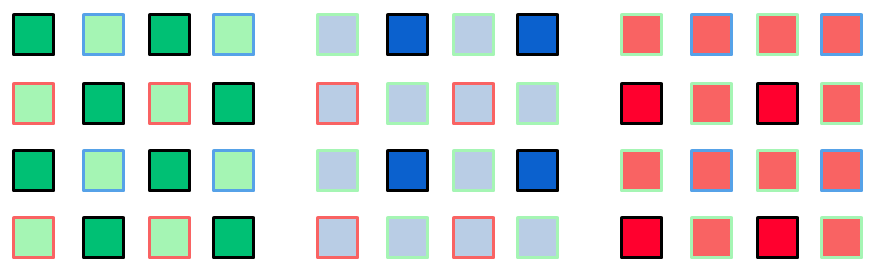
\includegraphics[width=0.9\textwidth]{Bayer2}
\caption{Descriptive diagram of the demosaicking to create the RGB channels from the Bayer pattern image.}
\end{figure}

The dark boxes in Figure \ref{Bayer2} represent the captured pixel while the lighter boxes are the interpolated locations, with their border showing what color was captured there. Again, there are twice as many green values as blue and red, but all three values are used at their captured spatial locations and then are interpolated to create a three channel RGB image.

Demosaicking is a well-understood and well-researched topic of interest where theories are being developed and applied to improve the interpolation results. The point to grasp here is that color imagery, even before any image processing algorithms are applied, is a sampled, quantized, and interpolated array of data. This shows a significant limitation in the strict accuracy of the initial information within a digital color image. While by no means a crippling factor, understanding this process allows for developing more scientifically stringent arguments for the concessions made later on in the development of the algorithm. For example, given this initial information loss in image capture, multiple-views are developed from statistically (randomly varied) quantized projections of the scene. Parallax and occlusion variations will occur with views at different spatial locations, but this also shows that intensity and color variations will occur in spite of any spatial variation. The views are inherently non-identical in terms of intensity/color, even when capturing the exact same object at the exact same depth and angle. This will be developed further as an important concept of usefulness of limitations on the metric for the algorithm. There will be many assumptions and simplifications presented as part of the development of this algorithm, and by understanding them as progressing in a foundational manner, starting with the imaging system itself, a clear and applicable argument for the development of this algorithm will be presented.

Therefore, at this stage, a digital image is seen initially as the demosaicked (interpolated) result of the Bayer pattern image. Stemming from that, a digital image is understood as a rigid, rectangular array of variable bit and channel depth. The number of channels pertains to the color range and the bit depth pertains to the intensity range. Standard contemporary color images are 3-channel (RGB) arrays of the notational size: $\mathfrak{m}\times\mathfrak{n}\times\mathfrak{p}$ (rows-by-columns-by-channels), and have a per pixel bit-depth of 8-bits, resulting in the descriptor of a 24-bit (3-channels with 8-bits each) color image. Variations of these characteristics exist in widespread use, and are important to understand, but the fundamental developments being made here can be built off of these criteria and easily translated to other image color-types and bit depths, thus all images in the rest of this work will be assumed 8 bits-per-pixel (bpp) and RGB images. But, the most fundamentally important concept in order to maintain a successful grasp of image processing is the notion that a digital image of size $\mathfrak{m} \times \mathfrak{n} \times \mathfrak{p}$ is akin to a $\mathfrak{p}$-dimensional discrete-space random function.

Stepping back to the notion of an $\mathfrak{m} \times \mathfrak{n} \times 1$, henceforth $\mathfrak{m} \times \mathfrak{n}$, image, the functional definition of this image will be: $f(x,y)$. In the image space, $x$ refers to the column-axis and $y$ refers to the row-axis, meaning that the pixel location $(y_{i},x_{j} )=(3,4)$ equates to row 4 and column 3, starting from the top left (as per the MATLAB� conventions). Now, $x$ and $y$ are not random vectors, they are independent vectors in either the image (frame) domain in the integer ranges: $[1,m]$ and $[1,n]$ (again following MATLAB� notation for consistency with the implementation), or in the global image (scene) rational domain with ranges: $(-\infty,\infty)$ and $(-\infty,\infty)$. The world function (for the scene) will be denoted as $\tilde{f}(\tilde{x},\tilde{y})$, and is understood as a continuous function of the continuous space. Thus the digital image (a frame from the view of the scene) is known as an approximation of the theoretical real world random function (the proposed model of the scene), as mentioned previously. The approximating function�s discrete result (the sampled and quantized projection of $\tilde{f}$), referred to for simplicity as the intensity value, is a discrete random variable dependent upon $x$ and $y$. This means that at any point $(x_{i},y_{j})$ in the domain has an intensity value of: 

\begin{equation}
\label{}
f(x_{i},y_{j}) \quad \vert \quad \{ x_{i} \epsilon [0,M), y_{j} \epsilon [0,N) \}
\end{equation}

And so, $f(x_{i},y_{j})$ is understood to be a discrete random variable characterized by its probability mass function (PMF), a sampled version of the real-world scene's modeled probability density function (PDF). Therefore the convention used in the rest of this discussion will refer to each image as numerated instances of $f$, the random variable denoting the intensity image function (e.g. $f_{1},f_{1},f_{1}, ...$). This 2-dimensional (2-D) PMF of the intensity is discrete, and for digital images it is accepted in practice as the normalized intensity histogram. The next section will discuss the relationship between the image histogram and the proposed PMF, which will be used to characterize an image (and its corresponding scene).



%%%%%%%%%%%%%%%%%%%%%%%%%%%%%%%%%%%%%%%%%%%%%%%%%%%%%%%%%%%%%%%%%%%%%%%%%%%%%%%
% END OF DOCUMENT

